%%%%%%%%%%%%%%%%%%%%%%%%%%%%% Define Article %%%%%%%%%%%%%%%%%%%%%%%%%%%%%%%%%%
\documentclass{article}   % two side printing
%%%%%%%%%%%%%%%%%%%%%%%%%%%%%%%%%%%%%%%%%%%%%%%%%%%%%%%%%%%%%%%%%%%%%%%%%%%%%%%

%%%%%%%%%%%%%%%%%%%%%%%%%%%%% Using Packages %%%%%%%%%%%%%%%%%%%%%%%%%%%%%%%%%%
\usepackage{geometry}
\usepackage{graphicx}
\usepackage{amssymb}
\usepackage{amsmath}
\usepackage{amsthm}
\usepackage{empheq}
\usepackage{mdframed}
\usepackage{booktabs}
\usepackage{lipsum}
\usepackage{color}
\usepackage{psfrag}
\usepackage{pgfplots}   % For plotting beautiful graphs
\usepackage{bm}
\usepackage[spanish]{babel}
\usepackage{biblatex} 
\usepackage{csquotes} 
\usepackage{setspace}
\usepackage{multicol}  
\usepackage[skip=3pt plus 1pt, indent=30pt]{parskip}    % Setting space between paragraphs and indent
\usepackage[T1]{fontenc}    % Output font encoding for international characters
\usepackage{helvet}        % Selecting font family
\usepackage{ragged2e}      % For text alignment
\usepackage{adjustbox}       % For defining new environments
\usepackage{fancyhdr}       % For defining headers and footers
\usepackage[cochineal]{newtxmath}
\usepackage{caption}
\usetikzlibrary{intersections}
\usetikzlibrary{decorations.text}
\usetikzlibrary{decorations.pathreplacing}
%%%%%%%%%%%%%%%%%%%%%%%%%%%%%%%%%%%%%%%%%%%%%%%%%%%%%%%%%%%%%%%%%%%%%%%%%%%%%%%

% Other Settings
\newcommand*{\freq}{\mathord{\mathit{f}}}
%\let\cleardoublepage=\clearpage
%\renewcommand{\baselinestretch}{1.5}
%%%%%%%%%%%%%%%%%%%%%%%%%% Page Setting %%%%%%%%%%%%%%%%%%%%%%%%%%%%%%%%%%%%%%%
\geometry{a4paper, textwidth=19cm, textheight=28.5cm, top=0.1cm, headheight=0.1cm}  % Setting page size
\graphicspath{{images/}}    % Setting path for images
\addbibresource{bibliography.bib}   % Setting path for bibliography
%%%%%%%%%%%%%%%%%%%%%%%%%% Define some useful colors %%%%%%%%%%%%%%%%%%%%%%%%%%
\definecolor{ocre}{RGB}{243,102,25}
\definecolor{mygray}{RGB}{243,243,244}
\definecolor{deepGreen}{RGB}{26,111,0}
\definecolor{shallowGreen}{RGB}{235,255,255}
\definecolor{deepBlue}{RGB}{61,124,222}
\definecolor{shallowBlue}{RGB}{235,249,255}
%%%%%%%%%%%%%%%%%%%%%%%%%%%%%%%%%%%%%%%%%%%%%%%%%%%%%%%%%%%%%%%%%%%%%%%%%%%%%%%

%%%%%%%%%%%%%%%%%%%%%%%%%% Define an orange box command %%%%%%%%%%%%%%%%%%%%%%%%
\newcommand\orangebox[1]{\fcolorbox{ocre}{mygray}{\hspace{1em}#1\hspace{1em}}}
%%%%%%%%%%%%%%%%%%%%%%%%%%%%%%%%%%%%%%%%%%%%%%%%%%%%%%%%%%%%%%%%%%%%%%%%%%%%%%%

%%%%%%%%%%%%%%%%%%%%%%%%%%%% English Environments %%%%%%%%%%%%%%%%%%%%%%%%%%%%%
\newtheoremstyle{mytheoremstyle}{3pt}{3pt}{\normalfont}{0cm}{\rmfamily\bfseries}{}{1em}{{\color{black}\thmname{#1}~\thmnumber{#2}}\thmnote{\,--\,#3}}
\newtheoremstyle{myproblemstyle}{3pt}{3pt}{\normalfont}{0cm}{\rmfamily\bfseries}{}{1em}{{\color{black}\thmname{#1}~\thmnumber{#2}}\thmnote{\,--\,#3}}
\theoremstyle{mytheoremstyle}
\newmdtheoremenv[linewidth=1pt,backgroundcolor=shallowGreen,linecolor=deepGreen,leftmargin=0pt,innerleftmargin=20pt,innerrightmargin=20pt,]{theorem}{Theorem}[section]
\theoremstyle{mytheoremstyle}
\newmdtheoremenv[linewidth=1pt,backgroundcolor=shallowBlue,linecolor=deepBlue,leftmargin=0pt,innerleftmargin=20pt,innerrightmargin=20pt,]{definition}{Definition}[section]
\theoremstyle{myproblemstyle}
\newmdtheoremenv[linecolor=black,leftmargin=0pt,innerleftmargin=10pt,innerrightmargin=10pt,]{problem}{Problem}[section]
%%%%%%%%%%%%%%%%%%%%%%%%%%%%%%%%%%%%%%%%%%%%%%%%%%%%%%%%%%%%%%%%%%%%%%%%%%%%%%%

%%%%%%%%%%%%%%%%%%%%%%%%%%%%%%% Plotting Settings %%%%%%%%%%%%%%%%%%%%%%%%%%%%%
\usepgfplotslibrary{colorbrewer}
\pgfplotsset{width=8cm,compat=1.9}
%%%%%%%%%%%%%%%%%%%%%%%%%%%%%%%%%%%%%%%%%%%%%%%%%%%%%%%%%%%%%%%%%%%%%%%%%%%%%%%

%%%%%%%%%%%%%%%%%%%%%%%%%%%%%%% Title & Author %%%%%%%%%%%%%%%%%%%%%%%%%%%%%%%%
\title{Implementación de un oscilador en ADS utilizando líneas de transmisión.}
\author{Luis Guillermo Macias Rojas}
%%%%%%%%%%%%%%%%%%%%%%%%%%%%%%%%%%%%%%%%%%%%%%%%%%%%%%%%%%%%%%%%%%%%%%%%%%%%%%%

%%%%%%%%%%%%%%%%%%%%%%%%%%%%%%% Header & Footer %%%%%%%%%%%%%%%%%%%%%%%%%%%%%%%
\pagestyle{fancy}  % Setting page style
\fancyhf{}
\fancyhead[L]{\text{Luis Guillermo Macias Rojas}}  % Setting header
%%%%%%%%%%%%%%%%%%%%%%%%%%%%%%%%%%%%%%%%%%%%%%%%%%%%%%%%%%%%%%%%%%%%%%%%%%%%%%%

\begin{document}
    \maketitle

    \fontfamily{phv}\selectfont % Selecting font family
    \noindent
    \textbf{Resumen:} En este trabajo se explora la implementación de un oscilador a partir de una línea de transmisión modelada
    en ADS aprovechando el alto número de reflexiones que suceden cuando la carga y la fuente están desacopladas. Se observa que la
    prevalencia de las oscilaciones está directamente relacionada con la diferencia entre las impedancias de entrada y de salida en un
    punto, sin embargo no es posible obtener oscilaciones sostenidas debido a la atenuación que experimenta la onda de voltaje 
    al propagarse a través de la línea de transmisión. Para obtener oscilaciones sostenidas es necesario agregar un elemento
    activo que contribuya con una resistencia negativa y compense las pérdidas de la línea de transmisión.

    \noindent\begin{minipage}{0.49\textwidth}   %uses 60% of the page
        %\vspace{2 mm}
        {\centering\section*{\large Introducción}}

        El coeficiente de reflexión determina la cantidad del voltaje incidente que va a ser reflejado al nodo anterior, está delimitado
        por la ecuación \eqref{eq:Gamma_dominio} y se puede calcular a partir de \eqref{eq:Gamma}.
        \begin{equation}
            \Gamma \in \mathbb{R} \quad : \quad -1 \leq \Gamma \leq 1
            \label{eq:Gamma_dominio}
        \end{equation}

        \begin{equation}
            \Gamma = \frac{Z_{L} - Z_{0}}{Z_{L} + Z_{0}} = \frac{V^{-}}{V^{+}} = \frac{V_{reflejado}}{V_{incidente}}
            \label{eq:Gamma}
        \end{equation}
        
        Haciendo que en todo momento se tenga un coeficiente de reflexión con magnitud igual a 1 sería posible implementar un 
        oscilador.

        \vspace{1 mm}
        {\centering\section*{\large Metodología}}
        La implementación de un oscilador a partir de una línea de transmisión requiere que $\Gamma_{L} = \Gamma_{S} = 1$, y para 
        cumplir con esta condición es necesario que $Z_{S} \gg Z_{0} \gg Z_{L}$. El esquemático de la figura \ref{fig:schematic} muestra el sistema
        realizado en ADS, en este se observa una resistencia de carga ($Z_{L}$) de 50 $\Omega$, una impedancia caracteristica ($Z_{0}$) 
        de 500 k$\Omega$ y una impedancia de fuente ($Z_{S}$) de 5 G$\Omega$, es decir, se escala cada impedancia por un factor de 10000.

        \vspace{0.4 cm}
        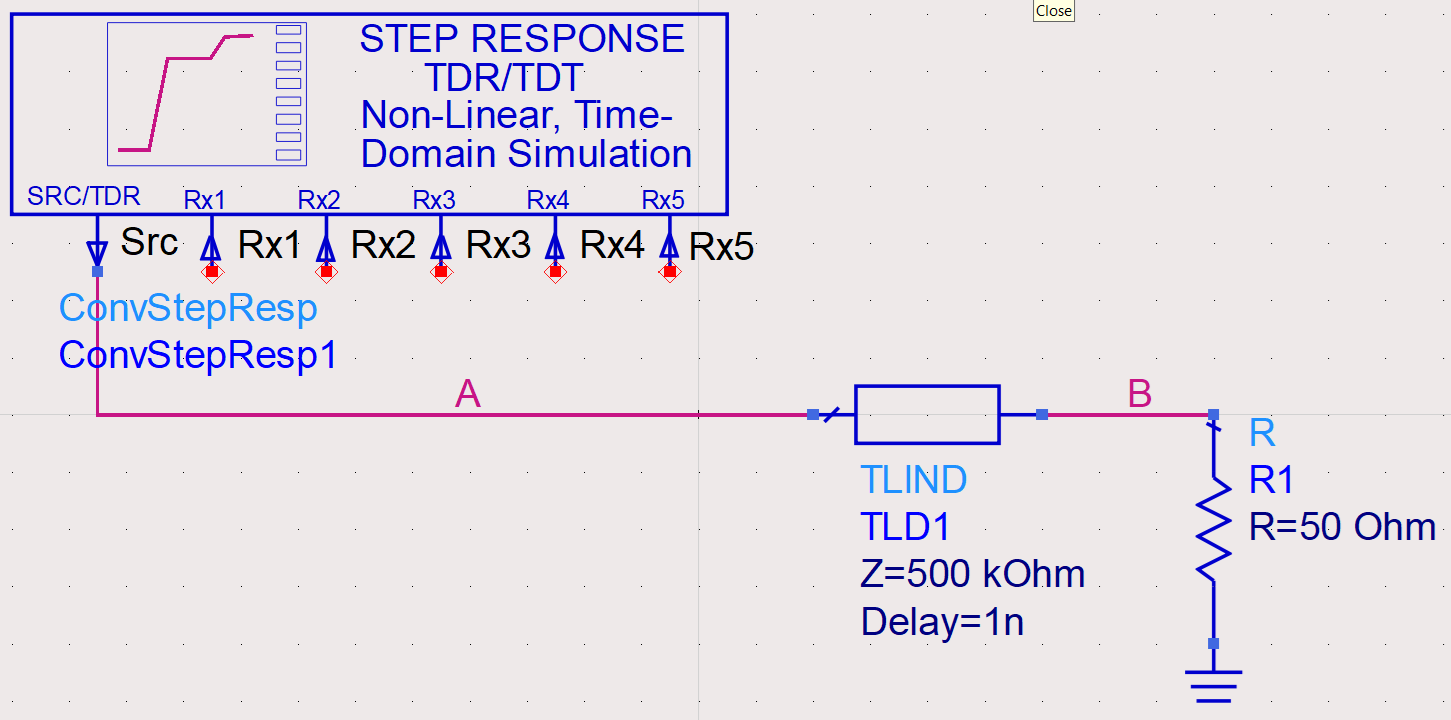
\includegraphics[width=\linewidth]{figures/schematic.png}
        \captionof{figure}{Esquemático de la linea de transmision.}
        \label{fig:schematic}
        \vspace{0.4 cm}

        El instrumento utilizado en esta simulación es un TDR/TDT, el cual actúa como una fuente de voltaje con una resistencia en
        serie ($Z_{S}$) que entrega un escalón de 1 V y analiza la respuesta transitoria del sistema.

        %\vspace{2 mm}
        {\centering\section*{\large Resultados}}
        Los resultados del análisis transitorio pueden observarse en la figura \ref{fig:Transient1}, en donde se muestra el voltaje
        incidente, el voltaje reflejado en la carga y el voltaje medido. Nótese como el voltaje reflejado es muy cercano a -1, lo cual
        indica que $|\Gamma_{L}| \approx 1$.

    \end{minipage}
    \hspace{0.38 cm}
    \begin{minipage}{0.49\textwidth}   %uses 50% of the page
        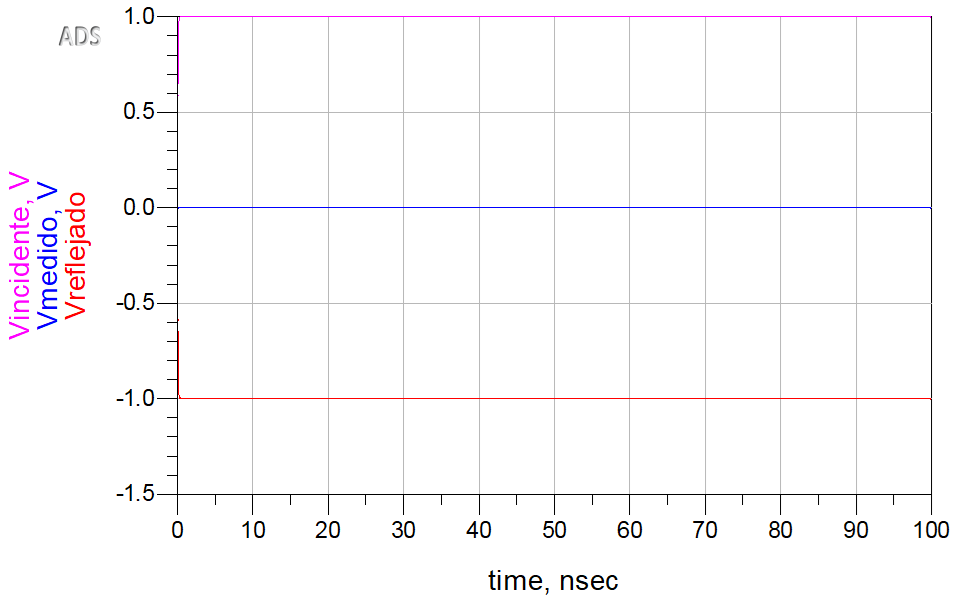
\includegraphics[width=\linewidth]{figures/Tran1.png}
        \captionof{figure}{Respuesta transitoria del sistema.}
        \label{fig:Transient1}

        La figura \ref{fig:Transient1} demuestra el correcto diseño de la línea de transmisión para que $\Gamma \approx 1$, sin embargo 
        no permite ver las oscilaciones del sistema debido a la baja amplitud de la señal, en la figura \ref{fig:Transient2} se observan
        estas oscilaciones durante 50 ciclos (100 reflexiones).
        
        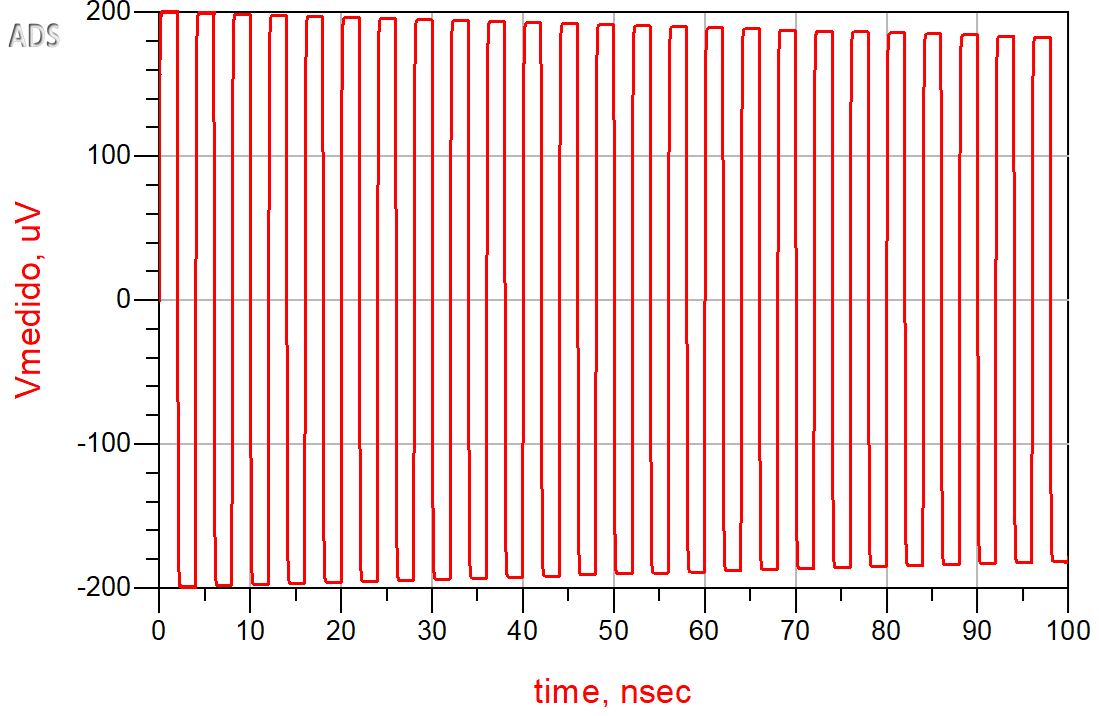
\includegraphics[width=\linewidth]{figures/Tran2.png}
        \captionof{figure}{Voltaje medido del oscilador.}
        \label{fig:Transient2}

        {\centering\section*{\large Conclusiones}}
        Es posible diseñar un oscilador LC utilizando líneas de transmisión y variando los coeficientes de reflexión, sin embargo, no es 
        posible obtener oscilaciones sostenidas debido a la atenuación que sufre el sistema por las no idealidades de la línea. Para
        compensar esto es necesario incluir un elemento activo (p. ej, un transistor) que introduzca una resistencia negativa y elimine estas pérdidas.

    \end{minipage}
    %\printbibliography  % Print bibliography
\end{document}